%%%%%%%%%%%%%%%%%%%%%%%%%%%%% Define Article %%%%%%%%%%%%%%%%%%%%%%%%%%%%%%%%%%
\documentclass[tikz, margin=5mm]{standalone}
%%%%%%%%%%%%%%%%%%%%%%%%%%%%%%%%%%%%%%%%%%%%%%%%%%%%%%%%%%%%%%%%%%%%%%%%%%%%%%%
\usepackage{tkz-euclide}

\begin{document}

\begin{tikzpicture}

    \tkzInit[xmax=360,xstep=20,ymax=3,xmin=0,ymin=-3]
    \tkzGrid[]
    \tkzClip[space=1]
    \tkzDrawX[label=$\theta$]
    \tkzLabelX
    \tkzDrawY[label=$\rho$]
    \tkzLabelY
    \tkzDefPoints{315/0.707106781/A}
    \tkzDrawPoints(A)
    \tkzLabelPoints(A)

    \tkzDefPoints{135/-0.707106781/B}
    \tkzDrawPoints(B)
    \tkzLabelPoints(B)

\end{tikzpicture}

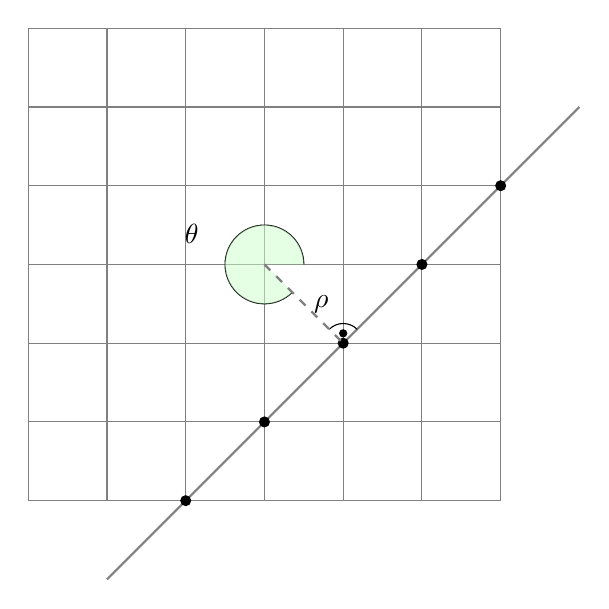
\begin{tikzpicture}

    \tkzInit[xmax=6,ymax=6,xmin=0,ymin=0]
    \tkzGrid[]
    \tkzAxeXY
    \draw[gray, thick] (1,-1) -- (7,5);

    \fill (2, 0)  circle[radius=2pt];
    \fill (3, 1)  circle[radius=2pt];
    \fill (4, 2)  circle[radius=2pt];
    \fill (5, 3)  circle[radius=2pt];
    \fill (6, 4)  circle[radius=2pt];

    \tkzDefPoints{3/3/O,4/2/B,5/3/A}
    \tkzMarkAngle[size=0.5](A,O,B)
    \tkzFillAngle[size=0.5,fill=green!20, opacity=0.5](A,O,B)
    \tkzLabelAngle(A,O,B){$\theta$}

    \tkzMarkRightAngle[german, size=0.25](A,B,O)

    \draw[gray, thick, dashed] (3,3) -- (4,2) node [midway, right, color=black] {$\rho$}; ;

\end{tikzpicture}


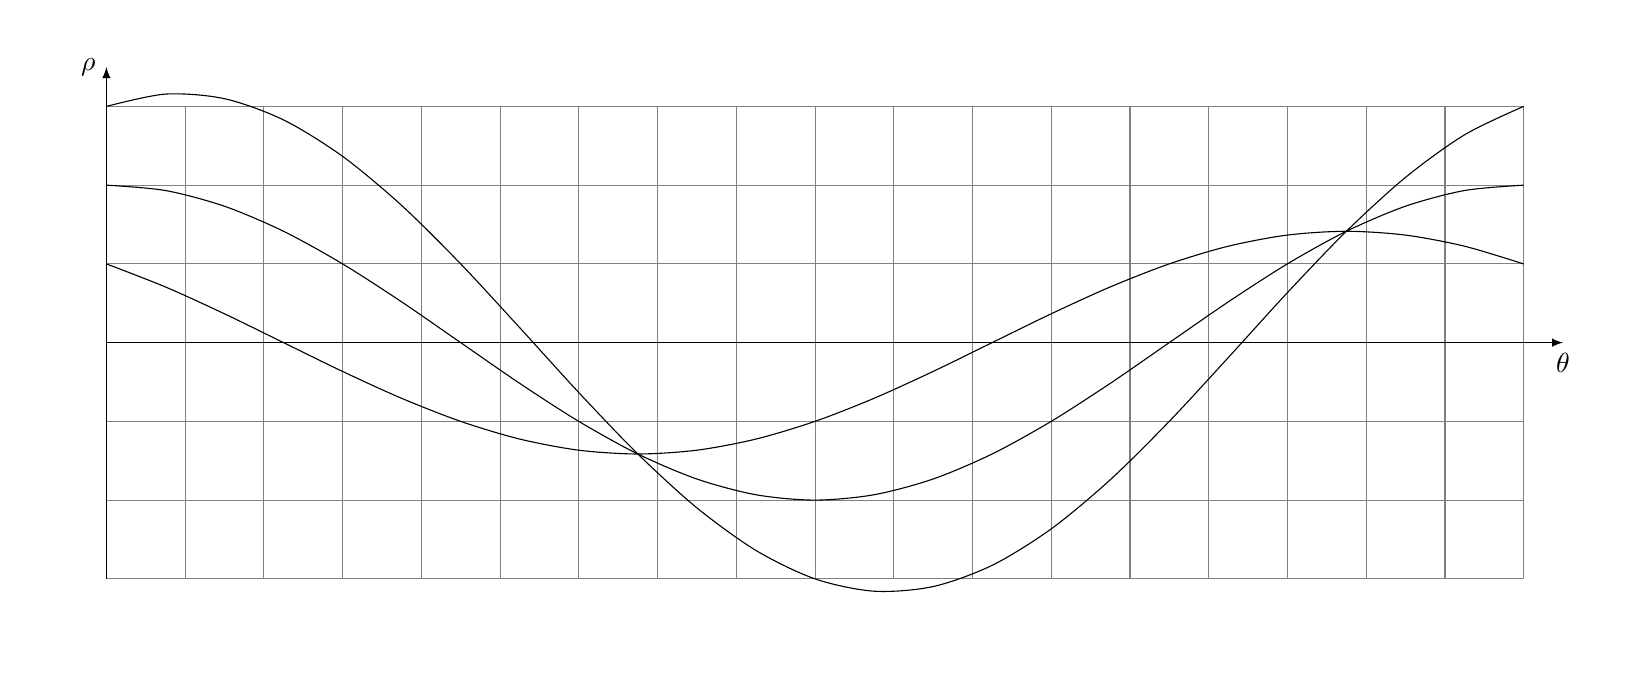
\begin{tikzpicture}

    \tkzInit[xmax=360,xstep=20,ymax=3,xmin=0,ymin=-3]
    \tkzGrid[]
    \tkzClip[space=1]
    \tkzDrawX[label=$\theta$]
    \tkzLabelX
    \tkzDrawY[label=$\rho$]
    \tkzLabelY

    \draw plot[domain=0:360/20,smooth] (\x,{1*cos(\x*20*0.0174532925 r) + -1*sin(\x*20*0.0174532925 r)});
    \draw plot[domain=0:360/20,smooth] (\x,{2*cos(\x*20*0.0174532925 r) + 0*sin(\x*20*0.0174532925 r)});
    \draw plot[domain=0:360/20,smooth] (\x,{3*cos(\x*20*0.0174532925 r) + 1*sin(\x*20*0.0174532925 r)});
\end{tikzpicture}

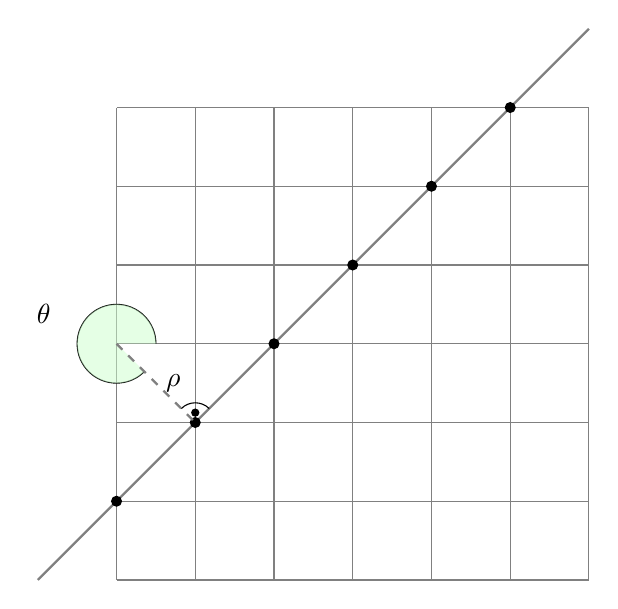
\begin{tikzpicture}

    \tkzInit[xmax=6,ymax=3,xmin=0,ymin=-3]
    \tkzGrid[]
    \tkzAxeXY
    \draw[gray, thick] (-1,-3) -- (6,4);
    \fill (0, -2)  circle[radius=2pt];
    \fill (1, -1)  circle[radius=2pt];
    \fill (2, 0)  circle[radius=2pt];
    \fill (3, 1)  circle[radius=2pt];
    \fill (4, 2)  circle[radius=2pt];
    \fill (5, 3)  circle[radius=2pt];

    \tkzDefPoints{0/0/O,1/-1/B,2/0/A}
    \tkzMarkAngle[size=0.5](A,O,B)
    \tkzFillAngle[size=0.5,fill=green!20, opacity=0.5](A,O,B)
    \tkzLabelAngle(A,O,B){$\theta$}

    \tkzMarkRightAngle[german, size=0.25](A,B,O)

    \draw[gray, thick, dashed] (0,0) -- (1,-1) node [midway, right, color=black] {$\rho$}; ;

\end{tikzpicture}

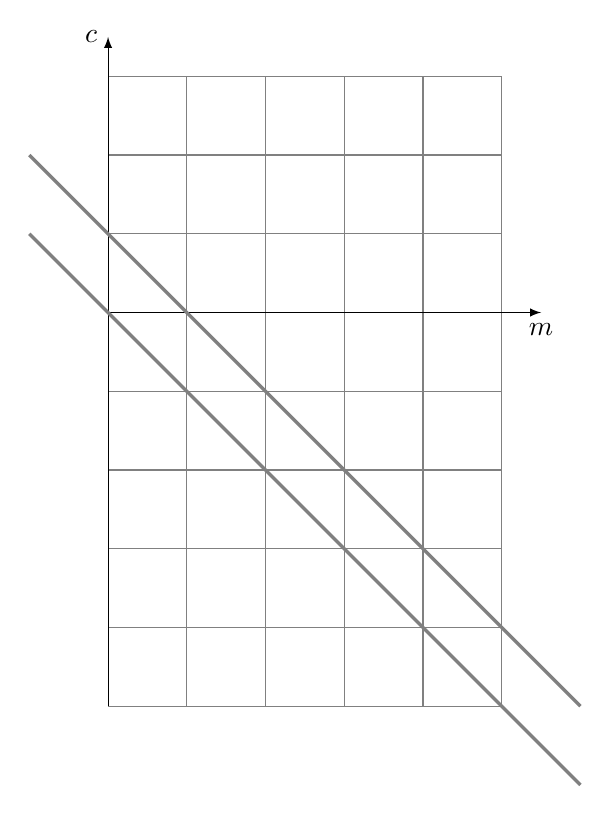
\begin{tikzpicture}

    \tkzInit[xmax=5,ymax=3,xmin=0,ymin=-5]
    \tkzGrid[]

    \tkzDrawX[label=$m$]
    \tkzLabelX
    \tkzDrawY[label=$c$]
    \tkzLabelY

    \draw[gray, very thick] (-1,1) -- (6, -6);
    \draw[gray, very thick] (-1,2) -- (6, -5);


\end{tikzpicture}

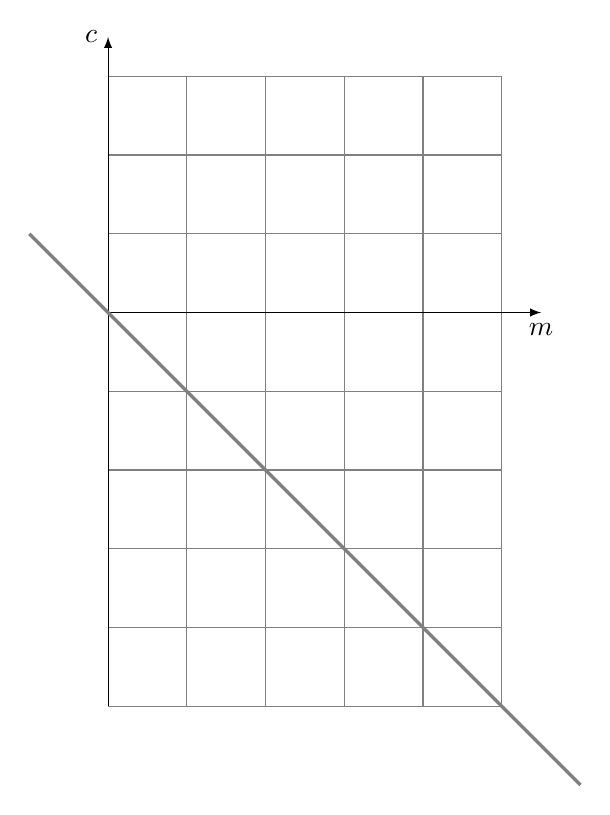
\begin{tikzpicture}

    \tkzInit[xmax=5,ymax=3,xmin=0,ymin=-5]
    \tkzGrid[]

    \tkzDrawX[label=$m$]
    \tkzLabelX
    \tkzDrawY[label=$c$]
    \tkzLabelY

    \draw[gray, very thick] (-1,1) -- (6, -6);


\end{tikzpicture}
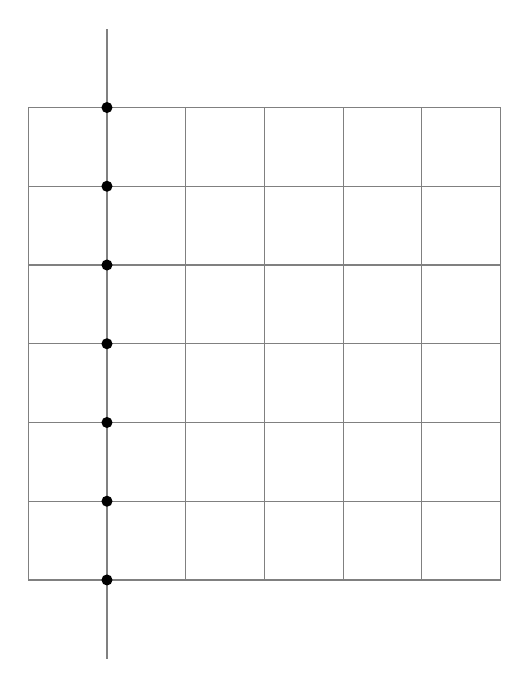
\begin{tikzpicture}

    \tkzInit[xmax=6,ymax=3,xmin=0,ymin=-3]
    \tkzGrid[]
    \tkzAxeXY
    \draw[gray, thick] (1,-4) -- (1,4);
    \fill (1, -1)  circle[radius=2pt];
    \fill (1, 0)  circle[radius=2pt];
    \fill (1, 1)  circle[radius=2pt];
    \fill (1, 2)  circle[radius=2pt];
    \fill (1, 3)  circle[radius=2pt];
    \fill (1, -2)  circle[radius=2pt];
    \fill (1, -3)  circle[radius=2pt];




\end{tikzpicture}

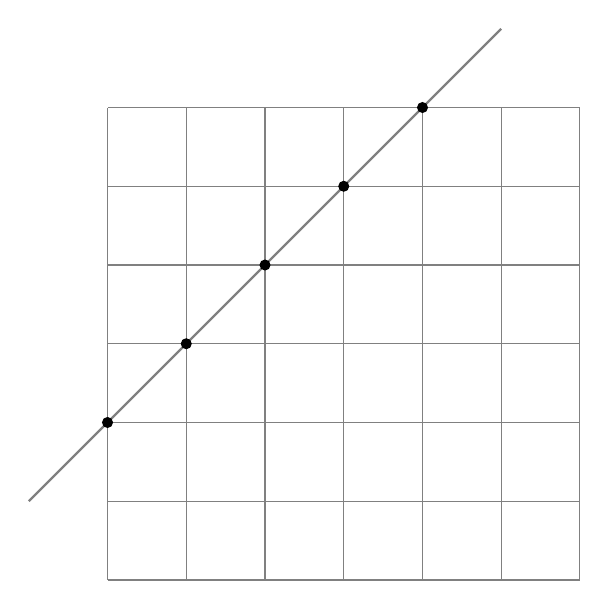
\begin{tikzpicture}

    \tkzInit[xmax=6,ymax=3,xmin=0,ymin=-3]
    \tkzGrid[]
    \tkzAxeXY
    \draw[gray, thick] (-1,-2) -- (5,4);
    \fill (0, -1)  circle[radius=2pt];
    \fill (1, 0)  circle[radius=2pt];
    \fill (2, 1)  circle[radius=2pt];
    \fill (3, 2)  circle[radius=2pt];
    \fill (4, 3)  circle[radius=2pt];




\end{tikzpicture}
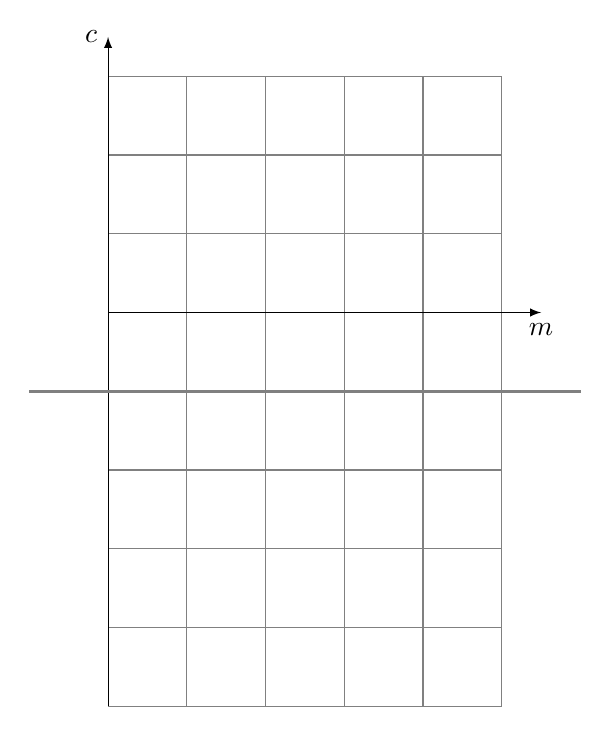
\begin{tikzpicture}

    \tkzInit[xmax=5,ymax=3,xmin=0,ymin=-5]
    \tkzGrid[]

    \tkzDrawX[label=$m$]
    \tkzLabelX
    \tkzDrawY[label=$c$]
    \tkzLabelY

    \draw[gray, very thick] (-1,-1) -- (6, -1);

\end{tikzpicture}

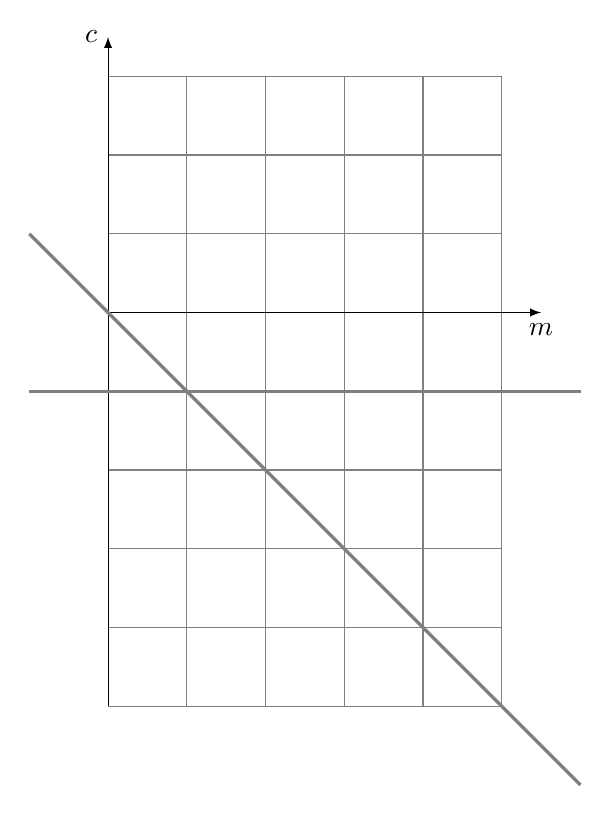
\begin{tikzpicture}

    \tkzInit[xmax=5,ymax=3,xmin=0,ymin=-5]
    \tkzGrid[]

    \tkzDrawX[label=$m$]
    \tkzLabelX
    \tkzDrawY[label=$c$]
    \tkzLabelY

    \draw[gray, very thick] (-1,-1) -- (6, -1);
    \draw[gray, very thick] (-1,1) -- (6, -6);


\end{tikzpicture}

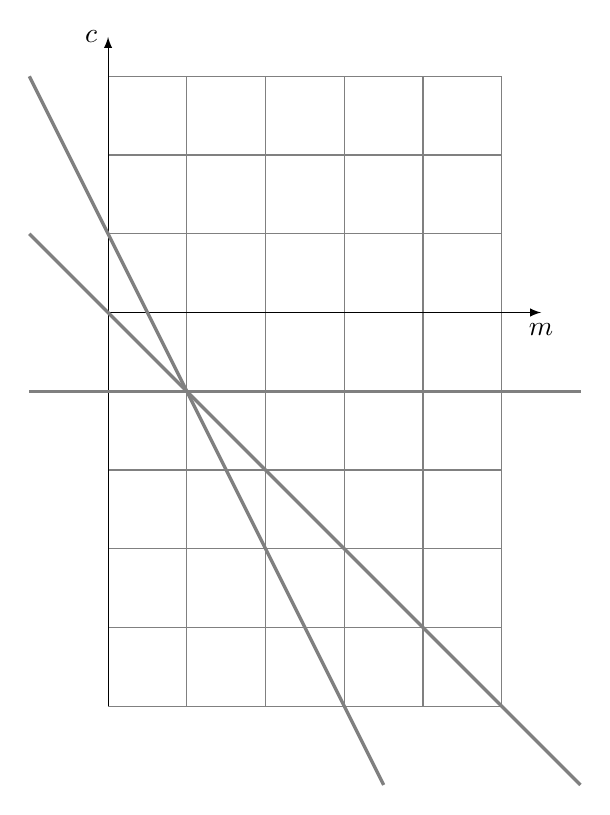
\begin{tikzpicture}

    \tkzInit[xmax=5,ymax=3,xmin=0,ymin=-5]
    \tkzGrid[]

    \tkzDrawX[label=$m$]
    \tkzLabelX
    \tkzDrawY[label=$c$]
    \tkzLabelY

    \draw[gray, very thick] (-1,-1) -- (6, -1);
    \draw[gray, very thick] (-1,1) -- (6, -6);
    \draw[gray, very thick] (-1,3) -- (3.5, -6);

\end{tikzpicture}

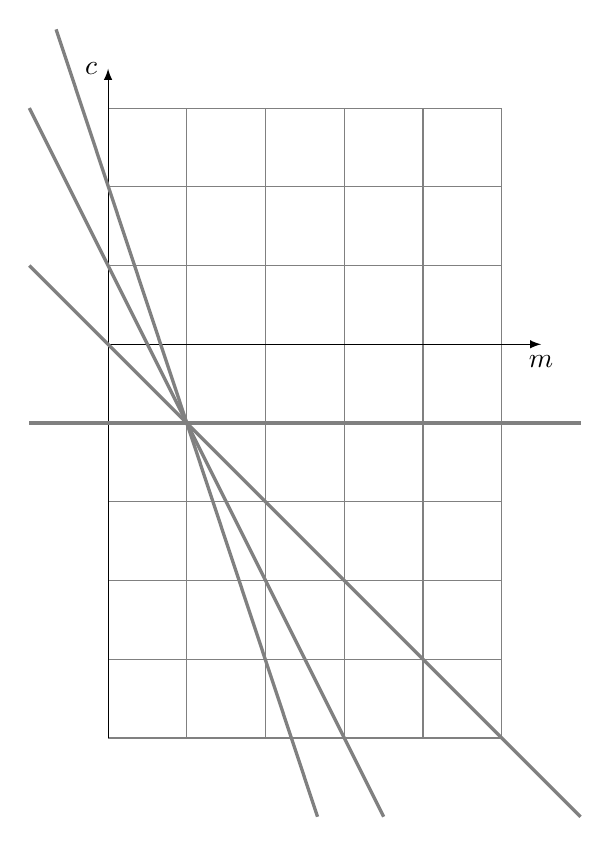
\begin{tikzpicture}

    \tkzInit[xmax=5,ymax=3,xmin=0,ymin=-5]
    \tkzGrid[]

    \tkzDrawX[label=$m$]
    \tkzLabelX
    \tkzDrawY[label=$c$]
    \tkzLabelY

    \draw[gray, very thick] (-1,-1) -- (6, -1);
    \draw[gray, very thick] (-1,1) -- (6, -6);
    \draw[gray, very thick] (-1,3) -- (3.5, -6);
    \draw[gray, very thick] (-0.66,4) -- (2.66, -6);

\end{tikzpicture}

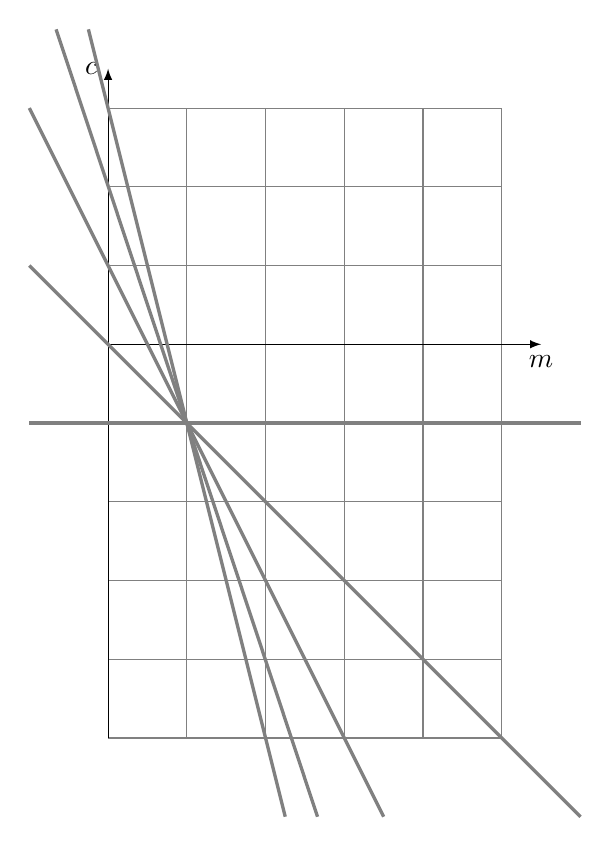
\begin{tikzpicture}

    \tkzInit[xmax=5,ymax=3,xmin=0,ymin=-5]
    \tkzGrid[]

    \tkzDrawX[label=$m$]
    \tkzLabelX
    \tkzDrawY[label=$c$]
    \tkzLabelY

    \draw[gray, very thick] (-1,-1) -- (6, -1);
    \draw[gray, very thick] (-1,1) -- (6, -6);
    \draw[gray, very thick] (-1,3) -- (3.5, -6);
    \draw[gray, very thick] (-0.66,4) -- (2.66, -6);
    \draw[gray, very thick] (-0.25,4) -- (2.25, -6);

\end{tikzpicture}

\end{document}